% =====================================================================
% Dissertation -- Condensed progress summary (Beamer), 5 pages
% Lineage-Aware Hierarchical Deep Learning for Imbalanced Multi-Class
% Classification of Peripheral Blood Cells
%
% Short form of Progress_Slides.tex: why the research is needed, the method,
% what is done, what comes next.
%
% Figures: ../../artifacts/ (generated) and ../assets/ (LaTeX figure deps).
% Needs Methodology-1.pdf alongside this file.
% Compile with: pdflatex Progress_Summary_Slides.tex   (run twice)
% =====================================================================
\documentclass[aspectratio=169,11pt]{beamer}

\usetheme{Madrid}
\usecolortheme{default}
\setbeamertemplate{navigation symbols}{}
\setbeamercovered{transparent}
\setbeamertemplate{itemize items}[circle]

\usepackage{graphicx}
\usepackage{booktabs}
\usepackage{xcolor}

\graphicspath{{../../artifacts/}{../assets/}{./}}

\setbeamerfont{block title}{size=\small}
\newcommand{\good}[1]{\textcolor{green!45!black}{\textbf{#1}}}
\newcommand{\bad}[1]{\textcolor{red!70!black}{\textbf{#1}}}

\title[Progress Summary]{Lineage-Aware Hierarchical Deep Learning for
Imbalanced Multi-Class Classification of Peripheral Blood Cells}
\subtitle{Progress summary}
\author{Arthiga Karthigesu}
\date{3 August 2026}

\begin{document}

% ---------------------------------------------------------------- Page 1
\begin{frame}{Why this research is needed}
  \begin{columns}[T]
    \begin{column}{0.55\textwidth}
      \scriptsize
      \textbf{The clinical problem}
      \begin{itemize}\setlength{\itemsep}{0.2em}
        \item Reading a blood smear is a core step in diagnosing blood
          disease, including leukaemia. An expert labels each cell by shape,
          chromatin, cytoplasm and granularity.
        \item The manual count is slow, repetitive, and varies between
          observers --- and it is hardest exactly where it matters, on the
          \textbf{rare and immature cells} whose appearance overlaps with
          their neighbours.
      \end{itemize}

      \smallskip
      \textbf{What existing systems get wrong}
      \begin{itemize}\setlength{\itemsep}{0.2em}
        \item They treat all 18 cell types as \textbf{flat, unrelated labels},
          discarding the known biology: cells belong to lymphoid, myeloid or
          erythroid lineages, and myeloid types lie on a maturation continuum.
        \item They report \textbf{plain accuracy}, which hides the failure that
          matters --- a model can score 96\% while missing most of the rarest
          class.
        \item Not all errors are equal: a \emph{within-lineage} confusion is
          clinically mild, a \emph{cross-lineage} one severe. Flat metrics
          cannot tell them apart.
      \end{itemize}
    \end{column}
    \begin{column}{0.43\textwidth}
      \centering
      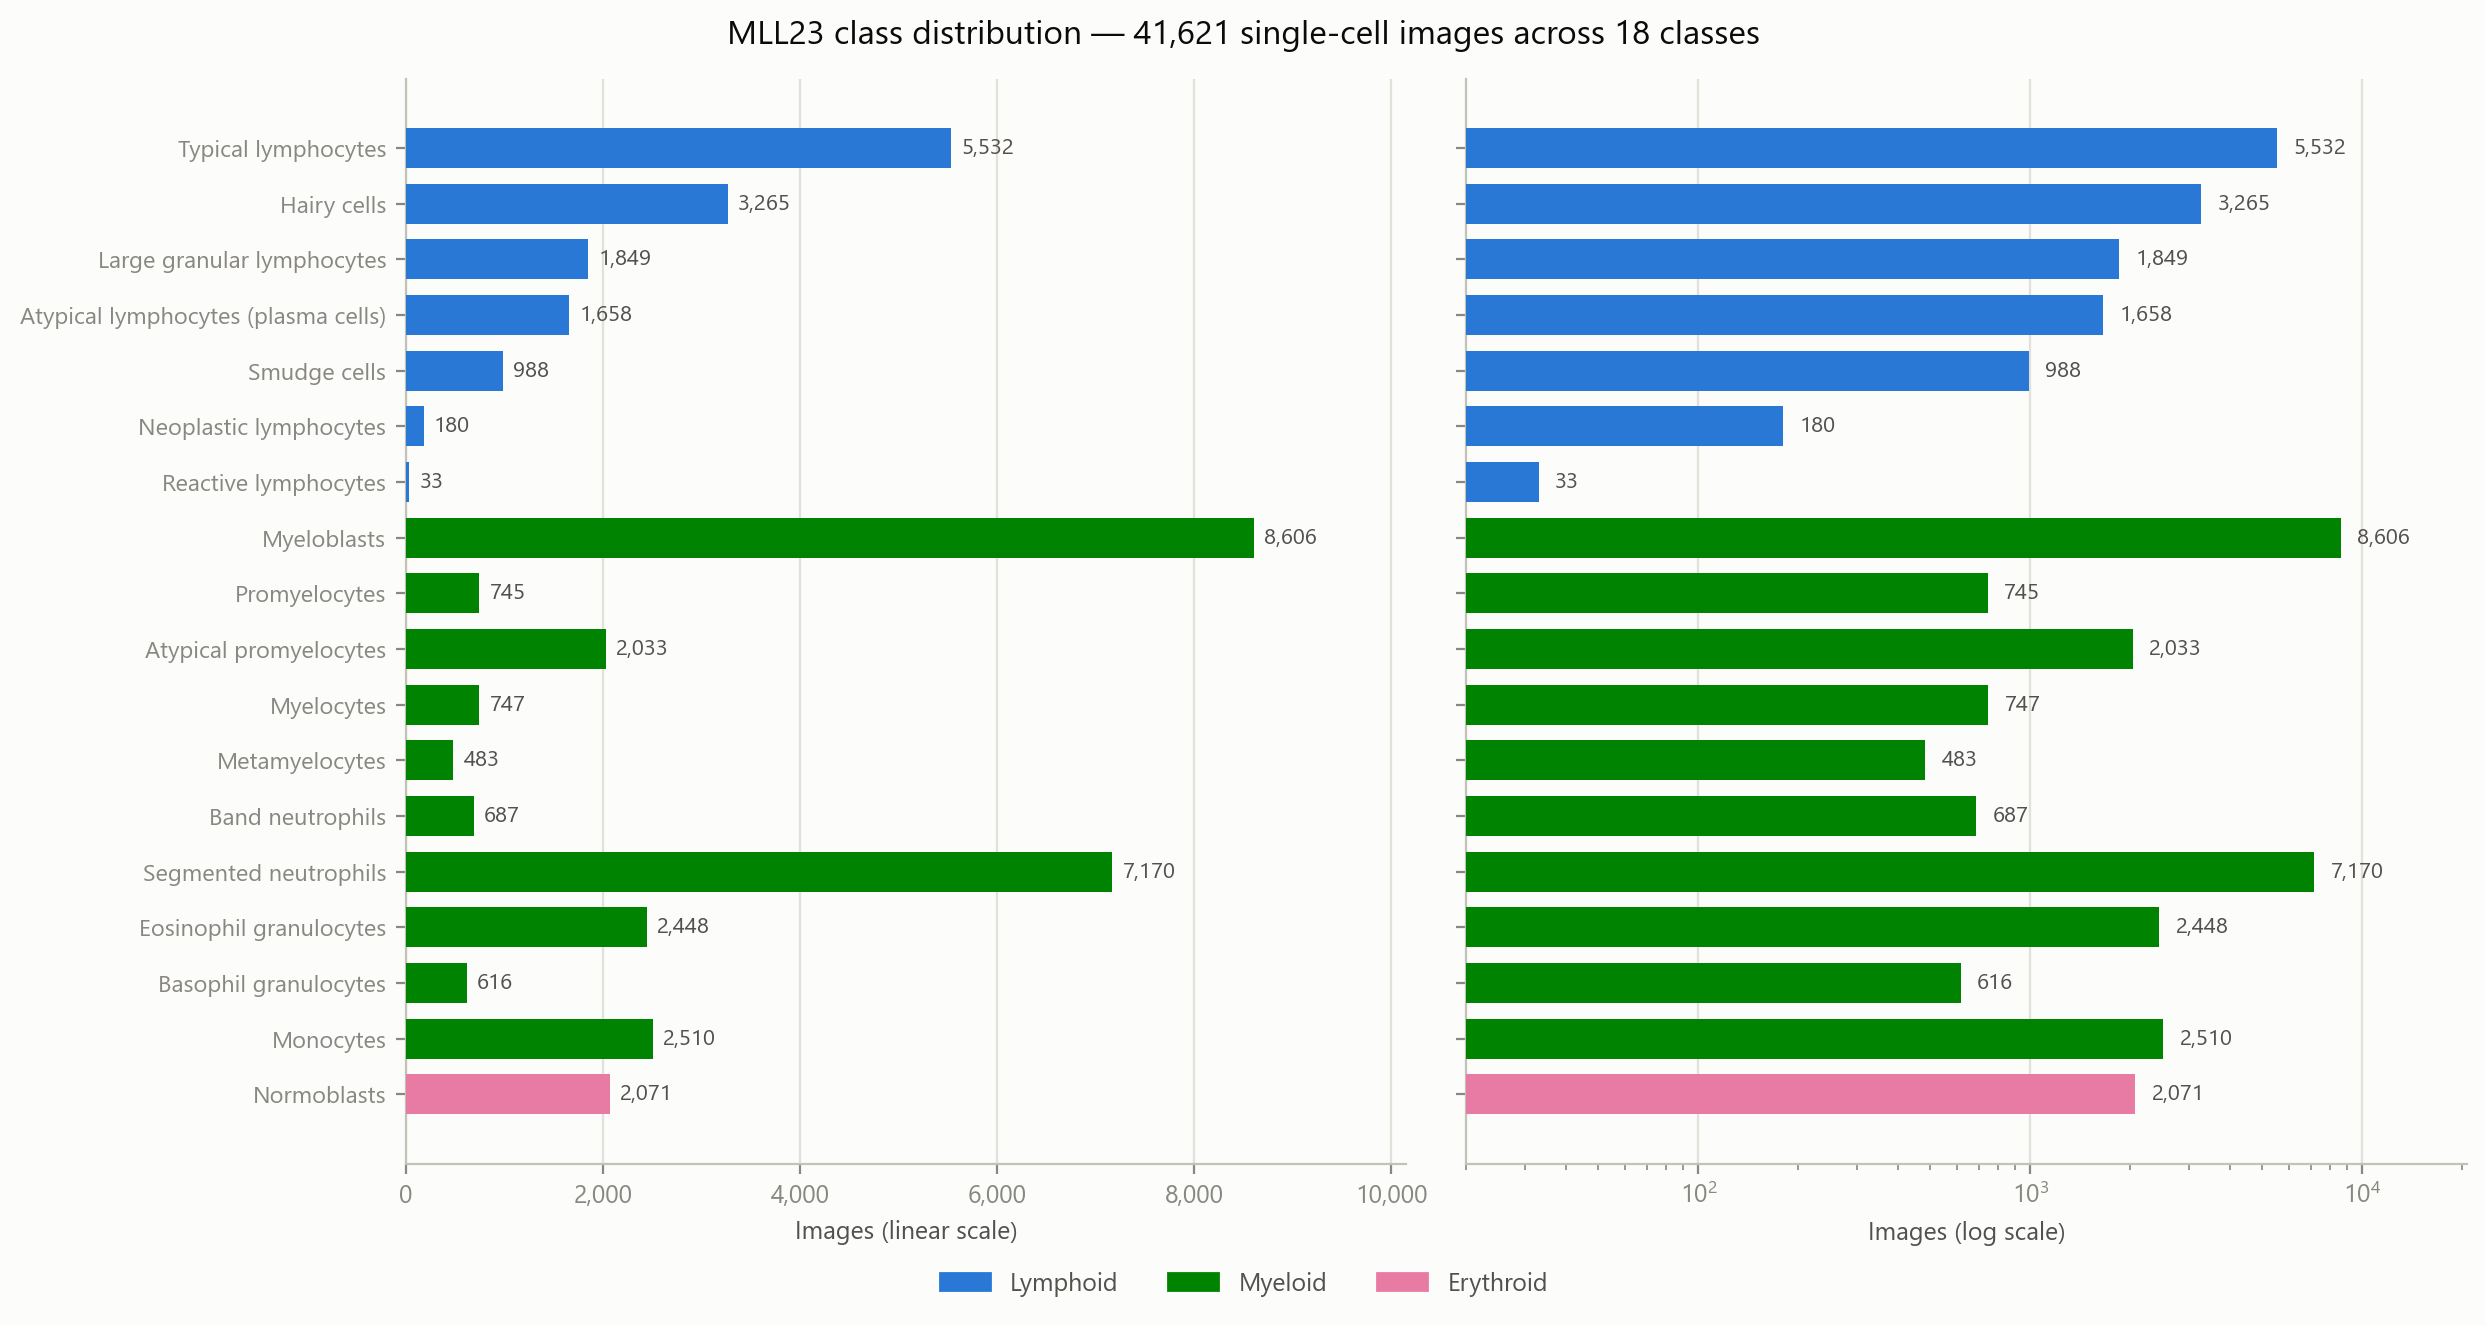
\includegraphics[width=0.98\linewidth]{class_distribution.png}

      {\scriptsize The imbalance is the subject, not an obstacle: \textbf{261:1}
      from myeloblasts (8,606) to reactive lymphocytes (33).\par}

      \vspace{0.3em}
      \begin{exampleblock}{Research question}
        \scriptsize
        Does a lineage-aware hierarchical classifier, with an imbalance-robust
        objective, improve fine-grained classification --- \textbf{especially
        for rare cell types} --- compared with a flat classifier on the same
        data?
      \end{exampleblock}
    \end{column}
  \end{columns}
\end{frame}

% ---------------------------------------------------------------- Page 2
\begin{frame}{The proposed method}
  \centering
  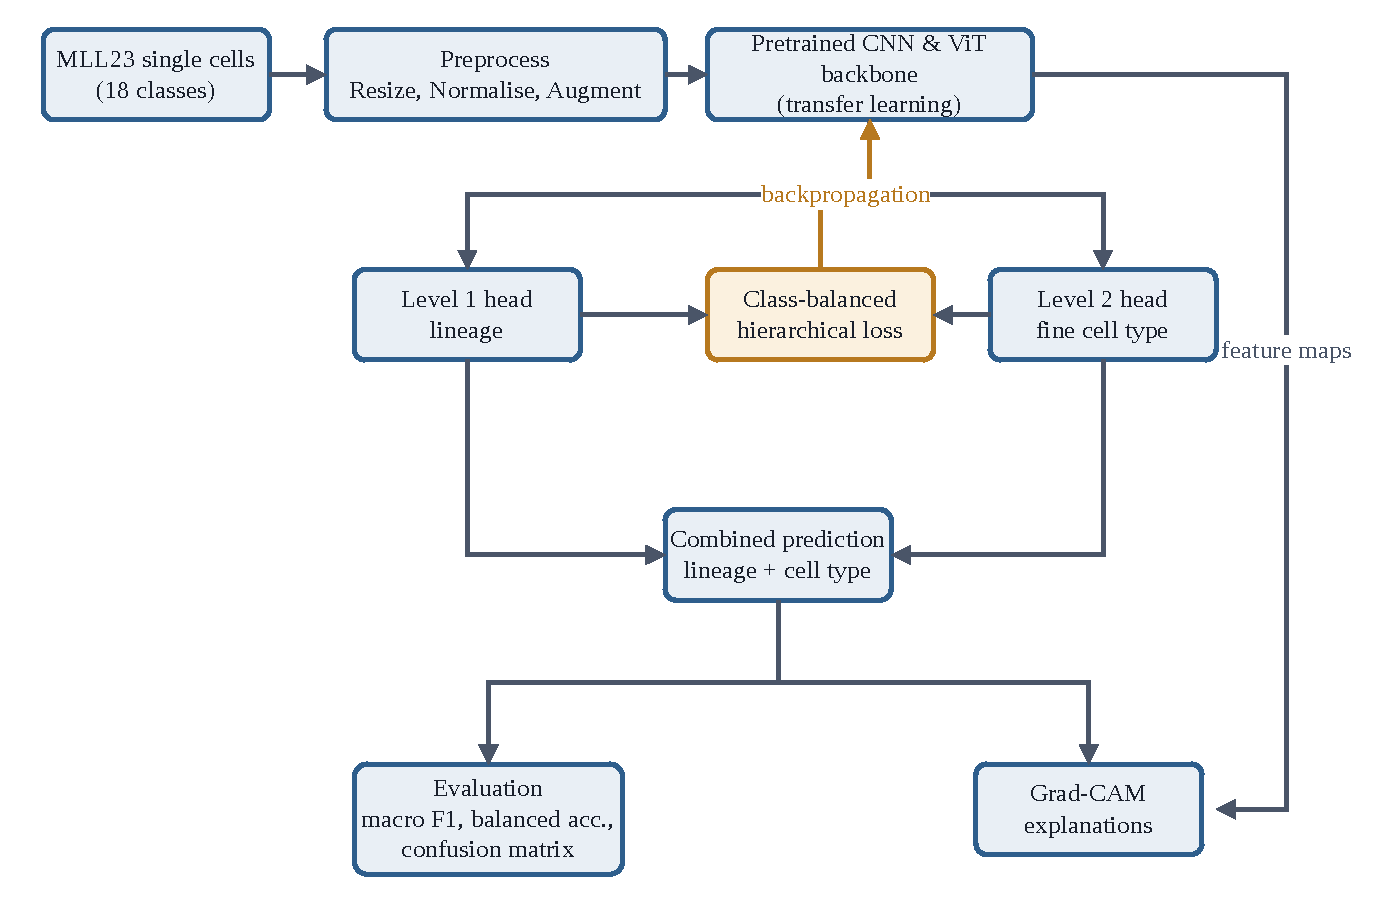
\includegraphics[width=0.52\linewidth]{Methodology-1.pdf}

  \vspace{0.4em}
  \begin{columns}[T]
    \begin{column}{0.47\textwidth}
      \begin{block}{Two heads, one backbone}
        \scriptsize
        Trained jointly, so rare types borrow strength from lineage
        neighbours. Lineage is a \textbf{regulariser, not a gate}.
      \end{block}
    \end{column}
    \begin{column}{0.47\textwidth}
      \begin{block}{What the arms switch off}
        \scriptsize
        One trainer, different flags: no lineage head $=$ \textbf{flat
        baseline}; no class-balanced/focal terms $=$ \textbf{imbalance ablation}.
      \end{block}
    \end{column}
  \end{columns}
\end{frame}

% ---------------------------------------------------------------- Page 3
\begin{frame}{What we have done}
  \begin{columns}[T]
    \begin{column}{0.47\textwidth}
      \scriptsize
      \textbf{Data and analysis} \good{complete}
      \begin{itemize}\setlength{\itemsep}{0.15em}
        \item 41,621 images acquired, checksum-verified, deterministic
          70/15/15 stratified split.
        \item Decoded-image cache: 178 $\rightarrow$ \good{$\sim$850 img/s}.
          Training was data-bound, not compute-bound.
        \item Exploratory finding: lineage structure is \textbf{local, not
          global} (silhouette $\approx 0$, but $k$-NN agreement $0.78$ vs
          $0.45$ chance) --- so lineage is used as a soft regulariser, not a
          routing gate.
      \end{itemize}

      \smallskip
      \textbf{Method} \good{complete}
      \begin{itemize}\setlength{\itemsep}{0.15em}
        \item Shared backbone $\rightarrow$ lineage head + fine head, trained
          jointly under a class-balanced hierarchical loss.
        \item One config-driven trainer runs every arm, so the ablations cannot
          drift apart. Grad-CAM and paired significance testing in place.
        \item Backbone screen selected \textbf{ViT}.
      \end{itemize}
    \end{column}
    \begin{column}{0.51\textwidth}
      \scriptsize
      \textbf{Results --- v2 matrix, ViT, 30 epochs} (8 of 12 runs)
      \smallskip

      \begin{tabular}{@{}lcccc@{}}
        \toprule
        \textbf{Arm} & \textbf{Seeds} & \textbf{Macro} & \textbf{Minority} & \textbf{Min.} \\
                     &                & \textbf{F1}    & \textbf{F1}       & \textbf{recall} \\
        \midrule
        Hierarchical (proposed) & 3 & \good{0.879} & \good{0.840} & \good{0.799} \\
        Flat baseline           & 3 & 0.874 & 0.823 & 0.776 \\
        No imbalance term       & 2 & 0.870 & \bad{0.771} & \bad{0.716} \\
        Stain-normalised        & 0 & \multicolumn{3}{c}{\emph{currently training}} \\
        \bottomrule
      \end{tabular}

      \smallskip
      \begin{itemize}\setlength{\itemsep}{0.15em}
        \item Proposed model wins on every metric, and by more on the rare
          classes ($+0.017$) than overall ($+0.005$) --- the predicted pattern.
          At $n=3$ seeds, \bad{not yet significant} ($p = 0.29$, $d_z = 0.84$).
        \item Removing the imbalance term costs \bad{$-0.069$} minority F1: that
          objective is the load-bearing component.
        \item The hierarchy is nearly \textbf{inert} --- lineage accuracy
          saturates at 98.9\%, so it regularises an axis already solved.
        \item v1 matrix \bad{invalidated} (run length drove the score,
          $r = +0.87$); protocol rebuilt, noise \good{$-54\%$}.
      \end{itemize}
    \end{column}
  \end{columns}
\end{frame}

% ---------------------------------------------------------------- Page 4
\begin{frame}{What we do next --- 1. Scale up the experiments}
  \begin{columns}[T]
    \begin{column}{0.55\textwidth}
      \scriptsize
      \begin{tabular}{@{}lcc@{}}
        \toprule
        \textbf{Work} & \textbf{Runs} & \textbf{Est.\ GPU} \\
        \midrule
        Finish the v2 matrix & 4 & ${\sim}5$ h \\
        \quad (\texttt{no\_imbalance} s2, \texttt{stain\_norm} $\times$3) & & \\
        Raise 3 $\rightarrow$ 5 seeds on all arms & 8 & ${\sim}10$ h \\
        Full backbone comparison at 30 epochs & 9 & ${\sim}12$ h \\
        \quad (ResNet / ConvNeXt / MobileNet $\times$3) & & \\
        \midrule
        \textbf{Total} & \textbf{21} & \textbf{${\sim}27$ h} \\
        \bottomrule
      \end{tabular}

      \medskip
      Spent so far: \textbf{16.6 GPU-hours} for 8 runs on an RTX 4070 Laptop.
    \end{column}
    \begin{column}{0.43\textwidth}
      \begin{block}{Why this is the priority}
        \scriptsize
        Three seeds gives \textbf{2 degrees of freedom}. The effect is real in
        direction and moderate-to-large in size, but the \emph{sample of runs}
        is too small to establish it. Five seeds, combined with the halved
        measurement noise, is what turns the paired tests from indicative into
        informative.
      \end{block}
      \begin{block}{Also outstanding}
        \scriptsize
        The 6-epoch screen \emph{selected} a backbone; it is not the backbone
        \emph{comparison} the proposal promised. Full-length runs are needed to
        report that honestly.
      \end{block}
      \begin{alertblock}{Decision needed}
        \scriptsize
        27 h is feasible locally but strictly serial. A rented cloud GPU would
        parallelise it into a weekend.
      \end{alertblock}
    \end{column}
  \end{columns}
\end{frame}

% ---------------------------------------------------------------- Page 5
\begin{frame}{What we do next --- 2. Fix the imbalanced-data problem}
  \footnotesize
  \begin{alertblock}{The problem, stated precisely}
    \scriptsize
    Minority recall is stuck at \textbf{0.80} --- one rare cell in five is still
    missed. Per-class F1 collapses on reactive lymphocytes ($\approx 0.55$,
    which leaves roughly \textbf{23 training images}) and on the adjacent
    myeloid maturation stages: metamyelocytes, myelocytes, band neutrophils
    ($0.59$--$0.72$). Class-balanced weights plus focal loss is a comparatively
    weak long-tail lever.
  \end{alertblock}

  \vspace{0.2em}
  Planned work, cheapest and highest-leverage first:
  \begin{enumerate}\setlength{\itemsep}{0.2em}
    \item \textbf{Decoupled training (cRT).} Learn the representation with
      instance-balanced sampling, then retrain \emph{only the classifier} with
      class-balanced sampling. Among the strongest long-tail methods, and it
      reuses the backbones already trained --- minutes per run, not hours.
    \item \textbf{Logit adjustment / LDAM margin loss.} Larger decision margins
      for rare classes; a drop-in replacement inside the existing
      \texttt{losses.py}.
    \item \textbf{Retarget the auxiliary task} at maturation stage within the
      myeloid branch, where the residual confusion actually lives, instead of at
      lineage --- which is already solved at 98.9\%.
  \end{enumerate}

  \vspace{0.3em}
  \begin{columns}[T]
    \begin{column}{0.49\textwidth}
      \begin{exampleblock}{Target}
        \scriptsize
        Minority macro F1 $0.840 \rightarrow 0.88+$ and minority recall off the
        $0.80$ plateau, with $p < 0.05$ at 5 seeds.
      \end{exampleblock}
    \end{column}
    \begin{column}{0.49\textwidth}
      \begin{block}{Sequence}
        \scriptsize
        Finish v2 matrix $\rightarrow$ add cRT and logit adjustment as new arms
        $\rightarrow$ re-run at 5 seeds $\rightarrow$ results chapter.
      \end{block}
    \end{column}
  \end{columns}
\end{frame}

\end{document}
